\section{Dynamické parametry obvodů v bipolárních technologiích}
- vstupní, výstupní a převodní charakteristiky

   \begin{figure}[h]
   \begin{center}
     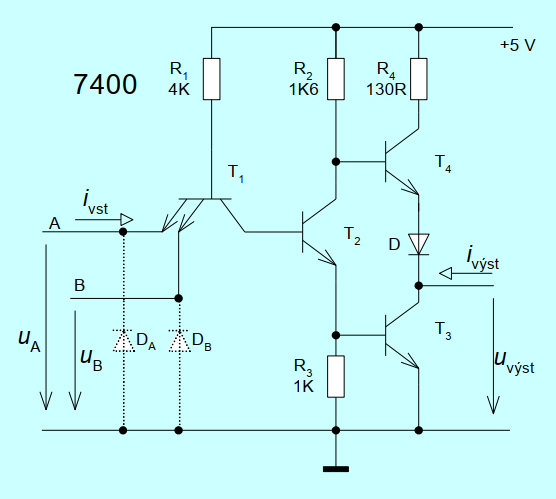
\includegraphics[scale=0.6]{images/NANDBJT.png}
   \end{center}
   \caption{Funkce NAND v BJT technologii}
  \end{figure}
 \subsection{Vstupní charakteristika}
 
    \begin{figure}[h]
   \begin{center}
     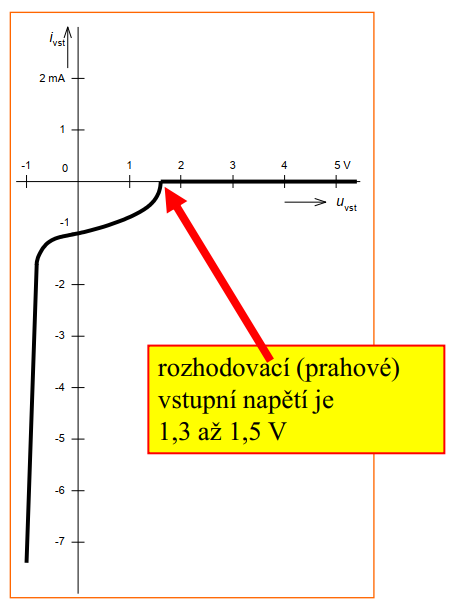
\includegraphics[scale=0.6]{images/VST.png}
   \end{center}
   \caption{Vstupní charakteristika}
  \end{figure}
 \subsection{Vstupní}
 
Tranzistor T2 uzavřen ic1= 0\\
vstupní proud:
\begin{equation}
i_{vst} = i_{b1} = \frac{U_{C}-u_{BE1}}{R_{1}}
\end{equation}

\textbf{Zvyšování vstupního napětí}\\
Tranzistor T2 se začíná otvírat, protože do jeho báze začíná vtékat proud při iVST = 0 mA veškerý proud rezistorem R1 teče do báze T2.\\
T2 a T3 v saturaci, uB2=(1,3 až 1,5) V\\
T1 přechází do inverzního režimu, při iVST = 0 mA bude mezi C a E minimální napětí, pro UT = 25 mV.\\

\textbf{Další zvyšování vstupního napětí:}\\
proud T1:
\begin{equation}
i_{vst} = \beta*i_{B1} = \frac{\beta*(U_{c}-3*u_{be})}{R_{1}}
\end{equation}
Při dalším zvyšování vstupního napětí se proud téměř nemění, až při napětí 7 až 8 V
dochází k průrazu přechodu emitor-báze T1, při kterém musí být vstupní proud omezen na
1 až 3 mA, proto maximální vstupní napětí udává výrobce 5,5 V.
\newpage
 \subsection{Výstupní charakteristika}
     \begin{figure}[h]
   \begin{center}
     \includegraphics[scale=0.6]{images/Vystup.png}
   \end{center}
   \caption{Výstupní charakteristika}
  \end{figure}

\subsubsection{U výstupní = 0 V; pro kladná napětí}
T3 nasycen, charakteristika iC3(uCE3) určuje průběh výstupní charakteristiky logického členu.\\
Malé výstupní proudy: uVÝST = uCES3 = 0,1 V při zvyšování výstupního proudu roste výstupní napětí\\
iVÝST = 140 mA přechází T3 z nasyceného do aktivního režimu => výstupní napětí prudce vzrůstá
\subsubsection{U výstupní = 0 V; pro záporná napětí}
v oblasti záporných napětí závisí průběh charakteristiky na vlastnostech substrátové diody mezi kolektorem T3 a společným vodičem.
\newpage
\subsubsection{Stav pro log. 1}  
     \begin{figure}[h]
   \begin{center}
     \includegraphics[scale=0.6]{images/Log1.png}
   \end{center}
   \caption{Stav pro logickou 1 na výstupu}
  \end{figure}
  
\newpage
 \subsection{Převodní charakteristika}
 \textbf{Tvar charakteristiky:}\\
Velikost napájecího napětí\\
Charakter připojené zátěže\\
Pracovní teplota obvodu\\

Šrafování vyznačuje zakázané oblasti, do kterých pro daná
vstupní napětí (uVSTL < 0,8 V a u VSTH > 2 V) nesmí výstupní napětí uVÝST zasáhnout
      \begin{figure}[h]
   \begin{center}
     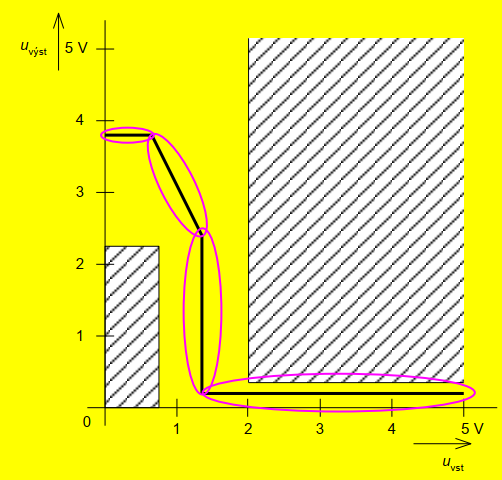
\includegraphics[scale=0.6]{images/Prevod.png}
   \end{center}
   \caption{Převodní charakteristika TTL}
  \end{figure}
  
a) malá vstupní napětí (0,6 až 0,8 V) → uVÝSTH = 3,3 až 3,7 V\\
b) při zvětšování uVST se otvírá T2 a jeho napěťové zesílení –R2/R3 = -1,4 udává
přibližně sklon převodní charakteristiky v oblasti klesajícího uVÝST\\  
c) při uVST = 1,3 V se začíná otevírat i výstupní tranzistor T3 a poněvadž je připojen paralelně k rezistoru R3 a jeho vstupní odpor RVST klesá, zvětšuje se zesílení T2 úměrně poměru - R2/(R3||RVST3), charakteristika je velmi strmá\\
d) další zvětšování uVST způsobí rychlý pokles výstupního napětí na hodnotu saturačního napětí výstupního tranzistoru T3, na výstupu členu je typické napětí uVÝSTL = 0,2 V\\
 
 
 
 
 
 
 
 
 
 
 
 
 
 
 
 
 
 
 
 
 
 
 
 
 
 
 
 
 
 
 














